\section{实验设计、结果与分析}
\label{sec:experiments}

本章回答四个研究问题。RQ1考察视觉证据对多模态验证器候选级判断能力的影响。RQ2检验复核系统能否在完整检测流程中纠正误报、漏检和错分类。RQ3分析复检门与接受门在不同调用预算下的效率和可靠性。RQ4考察配准扰动、差异表示和检测器替换对系统行为的影响。除专门说明的候选级诊断实验外，主结果均来自按模板组隔离的五折测试。正面发现、统计上不显著的结果和性能退化均纳入报告，整体结论不以单个折或单个预算点代替。

\subsection{实验设置}
\label{subsec:exp_setup}

\subsubsection{数据集及严格划分}

实验采用DeepPCB数据集\cite{tang2019deeppcb}。按仓库中的实际列表文件和图像文件核查，数据集包含1500对待检图与正常模板。官方\texttt{trainval}包含1000对，官方\texttt{test}包含500对。全部图像均为$640\times640$像素的JPEG图像，主体为单通道灰度图。1500个标注文件共包含10013个缺陷框。缺陷框分为open、short、mousebite、spur、spurious copper和pin-hole六类。每幅图的缺陷框数中位数为7。缺陷框宽度和高度的中位数分别为35和33像素。候选级复核处理的是局部细粒度目标，而非整图级异常。

官方划分不能直接支撑本文的主结论。数据目录可以稳定还原11个模板组，其中7个模板组同时出现在官方\texttt{trainval}和\texttt{test}中。同一模板组的板图会分别进入训练集和测试集，检测器因而接触到二者共享的板级结构。这种组间泄漏会低估跨模板泛化难度，并抬高检测和复核结果。本文仅用官方划分对照既有结果，不据此判断方法有效性。

主实验采用\texttt{GroupKFold}五折划分，以模板组作为不可拆分的分组单元。第$i$折的测试组在该折的训练和验证数据中完全不可见，验证集取下一折，其余三折用于训练检测器。评价第$i$折的门控模型时，只使用其余折产生的折外候选训练，防止门控阶段重新引入样本泄漏。11个模板组的规模从14对到325对不等，最大组与最小组相差23.21倍，因此各折样本量不能强行等分。表~\ref{tab:fold_composition}列出了实际测试组成，五折共覆盖1500对图像，每个图像对恰好作为测试样本一次。

\begin{table*}[t]
  \centering
  \caption{按模板组隔离的五折测试集组成}
  \label{tab:fold_composition}
  \setlength{\tabcolsep}{5pt}
  \begin{tabular}{clrr}
    \hline
    折 & 测试模板组 & 图像对数 & 占全部数据比例 \\
    \hline
    fold\_0 & group20085 & 325 & 21.67\% \\
    fold\_1 & group00041、group50600 & 300 & 20.00\% \\
    fold\_2 & group12300、group13000 & 314 & 20.93\% \\
    fold\_3 & group12000、group12100、group44000 & 260 & 17.33\% \\
    fold\_4 & group77000、group90100、group92000 & 301 & 20.07\% \\
    \hline
    合计 & 11个模板组 & 1500 & 100.00\% \\
    \hline
  \end{tabular}
\end{table*}

\subsubsection{基础检测器与多模态验证器}

基础检测器采用YOLOv8s。每折在三个训练折上训练，在独立验证折上选择F1最优工作点，并在测试折上输出折外预测。低置信度阈值0.001只用于计算mAP，不用于报告部署工作点的Precision、Recall和F1。五折检测器的mAP@0.5为$0.9580\pm0.0164$，mAP@0.5:0.95为$0.7135\pm0.0407$。验证集选定工作点上的Precision为$0.9264\pm0.0291$。Recall为$0.8964\pm0.0469$，F1为$0.9105\pm0.0312$。折间F1从0.8721到0.9522，反映了模板隔离后不同板型的难度差异。因此，结果同时报告均值和标准差。

多模态验证器只接收已经定位并放大的证据卡，不在整幅图上自由生成检测框。主后端为本机Codex CLI，模型为\texttt{gpt-5.6-sol}。推理强度设为low，并采用确定性解码。输入由当前紧裁剪、正常模板和上下文组成。JSON Schema将输出约束为固定字段；解析失败时，系统保持基础检测结果。默认协议隐藏检测器类别和置信度。验证器独立判断缺陷是否存在及其类别，系统再将判断映射为keep、remove、relabel或add。keep、remove和relabel始终作用于检测器原框。add只能接受已有差异候选，验证器没有任意造框权限。所有响应按候选、证据配置、模型和解码参数缓存，累计真实调用约7000次。12路并发下实测吞吐上限约26次每分钟，单候选平均墙钟时间约29秒。该成本要求系统选择性调用验证器。

\subsubsection{评价指标与统计方法}

常规检测指标包括Precision、Recall、F1、mAP@0.5、mAP@0.5:0.95和各类别AP。本文另定义五个指标衡量复核动作。设基础检测器的误报、漏检、错分类和正确检测数量分别为$N_{\mathrm{FP}}^0$、$N_{\mathrm{FN}}^0$、$N_{\mathrm{MC}}^0$和$N_{\mathrm{TP}}^0$。误报修正率FPCR是正确删除的原始误报数与$N_{\mathrm{FP}}^0$之比。漏检恢复率MDRR是新增匹配的原始漏检数与$N_{\mathrm{FN}}^0$之比。类别修正准确率MCCA是正确重分类数与$N_{\mathrm{MC}}^0$之比。正确检测保留率TPRR是复核后仍正确的原始TP数与$N_{\mathrm{TP}}^0$之比。有害修正率HCR是降低检测效用的已接受修改数与全部已接受修改数之比。TPRR衡量系统是否破坏原本正确的检测，HCR衡量已执行修改的风险。

成本指标包括验证器调用率、每图调用次数、单候选平均时延和P95时延、每图输入token数以及配准失败回退率。RQ1在同一批候选上比较不同证据配置。置信区间采用按图像聚类的bootstrap，避免把同一图像中的多个候选视为独立样本。RQ2对Full与基础工作点进行2000次按图像聚类的配对bootstrap。端到端指标报告五折均值与折间标准差。所有门控阈值均由验证折选择，并在测试前冻结。

\subsection{可纠错空间分析}
\label{subsec:correctable_space}

在评价复核方法之前，需要先确定基础检测器留下了哪些错误。本文按IoU匹配和类别一致性将工作点输出分解为正确检测、错分类、误报、漏检和纯定位错误。纯定位错误表示检测器已经对目标作出响应，但定位未达到正式匹配阈值。这类错误与三类可通过删除、新增或重分类动作直接处理的错误分开统计。表~\ref{tab:error_decomposition}给出五折结果。

\begin{table*}[t]
  \centering
  \caption{五折基础检测器错误分解}
  \label{tab:error_decomposition}
  \setlength{\tabcolsep}{7pt}
  \begin{tabular}{crrrrrr}
    \hline
    折 & TP & 错分类 & 误报 & 漏检 & 纯定位错误 & 可纠错空间 \\
    \hline
    fold\_0 & 2085 & 6  & 216 & 335 & 2  & 557 \\
    fold\_1 & 1987 & 9  & 166 & 77  & 1  & 252 \\
    fold\_2 & 1894 & 8  & 24  & 148 & 1  & 180 \\
    fold\_3 & 1608 & 23 & 134 & 118 & 10 & 275 \\
    fold\_4 & 1408 & 15 & 96  & 269 & 9  & 380 \\
    \hline
    合计 & 8982 & 61 & 636 & 947 & 23 & 1644 \\
    \hline
  \end{tabular}
\end{table*}

可纠错空间是错分类、误报和漏检之和，共1644项。漏检947项，占57.6\%，是最大错误来源。误报636项，占38.7\%；错分类61项，占3.7\%。只复核检测器已经提出的框，最多能处理误报和错分类，无法触及超过一半的潜在纠错空间。差异候选用于提出检测器未覆盖的位置，再由验证器决定是否新增。错分类的基数只有3.7\%，限制了重分类动作对总体F1的最高贡献。

折间分布同样不均衡。fold\_0有335个漏检和216个误报，可纠错空间为557。fold\_2只有180项可纠错错误，其中误报仅24个。单折结果会偏置复核收益和风险估计。五折隔离既防止模板泄漏，也覆盖不同的误报与漏检构成。RQ2的Oracle分析使用完整固定候选集计算候选覆盖上界，并区分“没有提出候选”与“候选已提出但验证器判断错误”。

\subsection{RQ1：证据消融}
\label{subsec:rq1}

RQ1固定候选、模型、提示词骨架和解码参数，只改变证据卡内容。A0仅给出当前紧裁剪，A1加入上下文，A2再加入配对正常模板。A3和A4分别加入外观差异与拓扑差异，A5和A6组合更多证据。七组主消融及四组附加对照均在相同的200个候选上评价。候选级任务判断候选位置是否存在真实缺陷。F1相对A0的差值采用按图像聚类的bootstrap计算95\%置信区间。该诊断集用于比较证据，不用于估计自然部署时的缺陷发生率。

\begin{table*}[t]
  \centering
  \caption{RQ1主证据消融结果，$n=200$}
  \label{tab:rq1_main}
  \setlength{\tabcolsep}{6pt}
  \begin{tabular}{clrrlc}
    \hline
    配置 & 证据设置 & F1 & 相对A0 & 95\%置信区间 & 显著性 \\
    \hline
    A0 & 仅当前裁剪 & 0.6375 & 0.0000 & 基准 & 不适用 \\
    A1 & 加上下文 & 0.7033 & +0.0658 & [+0.0007, +0.1244] & 边界显著 \\
    A2 & 加正常模板 & 0.7553 & +0.1178 & [+0.0259, +0.2304] & 是 \\
    A3 & 加外观差异 & 0.7380 & +0.1005 & [+0.0304, +0.1920] & 是 \\
    A4 & 加拓扑图 & 0.7571 & +0.1196 & [+0.0280, +0.2390] & 是 \\
    A5 & 组合证据 & 0.7079 & +0.0704 & [-0.0168, +0.1821] & 否 \\
    A6 & 完整证据卡 & 0.7347 & +0.0972 & [-0.0012, +0.2254] & 否 \\
    \hline
  \end{tabular}
\end{table*}

表~\ref{tab:rq1_main}显示，A2相对A0提高0.1178，置信区间为[+0.0259,+0.2304]。正常模板带来的增量有统计支持。A3和A4相对A0也显著。A4的F1为0.7571，略高于A2的0.7553，但相对A2的差异处于置信区间内，未证明拓扑图带来增量。A5和A6相对A0分别提高0.0704和0.0972，置信区间均跨越0，因此不显著。结果不支持“证据越多，验证器判断越好”。当前实验也未检验更多视觉证据未产生增量的具体机制。

阶段B2排查外观热图的负结果是否源于渲染自动拉伸或配准残差，并在同一批150个候选上完成450次新调用。A2N保留当前裁剪、模板和上下文，只增加数值摘要。A2T只增加固定颜色的拓扑差异图。A6F将外观图改为按预先冻结阈值生成的二值图。实现核查确认原外观图使用全样本统一的$[0,1]$色标，不存在逐样本最小最大值拉伸。表~\ref{tab:rq1_b2}中，三个专门对照均低于同批候选上的A2，最高的A6F也低0.0304。数值摘要没有产生增益，二值化也没有挽回完整证据卡。因此，负结果不能归结为单一显示错误。

\begin{table}[t]
  \centering
  \caption{阶段B2专门对照结果，$n=150$}
  \label{tab:rq1_b2}
  \setlength{\tabcolsep}{5pt}
  \begin{tabular}{lrrr}
    \hline
    配置 & F1 & uncertain率 & JSON解析率 \\
    \hline
    A2  & 0.8082 & 0.1067 & 1.0000 \\
    A2N & 0.7183 & 0.1133 & 1.0000 \\
    A2T & 0.7481 & 0.2400 & 1.0000 \\
    A6F & 0.7778 & 0.1800 & 1.0000 \\
    A6  & 0.7763 & 0.1133 & 1.0000 \\
    \hline
  \end{tabular}
\end{table}

表~\ref{tab:rq1_controls}报告四组提示协议对照。去掉“配准不可靠”警告的A6\_no\_reg\_warning取得最高F1 0.8000。该警告没有带来预期的稳健性，但实验未单独检验其作用机制。向验证器提供检测器标签的A6\_label\_aware达到0.7701，高于隐藏标签的A6 0.7347。本实验没有证明去锚定优于标签可见协议。旧提示词A6\_prompt\_v1达到0.7678，其normal判定率为0.31，低于新版的0.39。提示版本改变了判定倾向。自由文本A6\_free\_text的F1为0.6813，JSON可解析率为0，必须依赖后处理启发式。固定Schema是执行复核动作的必要约束。

\begin{table}[t]
  \centering
  \caption{RQ1四组附加对照}
  \label{tab:rq1_controls}
  \setlength{\tabcolsep}{4pt}
  \begin{tabular}{lrr}
    \hline
    配置 & F1 & JSON解析率 \\
    \hline
    A6\_no\_reg\_warning & 0.8000 & 1.0000 \\
    A6\_label\_aware & 0.7701 & 1.0000 \\
    A6\_prompt\_v1 & 0.7678 & 1.0000 \\
    A6\_free\_text & 0.6813 & 0.0000 \\
    \hline
  \end{tabular}
\end{table}

图~\ref{fig:per_class_evidence_gain}给出六类缺陷上的证据增益。各类别没有呈现“完整证据一致占优”的模式，宏平均性能也受类别混淆影响。RQ2和RQ3据此固定采用A2，只向验证器展示当前紧裁剪、正常模板和上下文。8维拓扑向量保留为复检门和接受门的结构化特征。当前实验不支持将其作为验证器视觉输入的增量。RQ1表明正常模板有效，完整外观与拓扑证据卡则未获支持。

\begin{figure}[t]
  \centering
  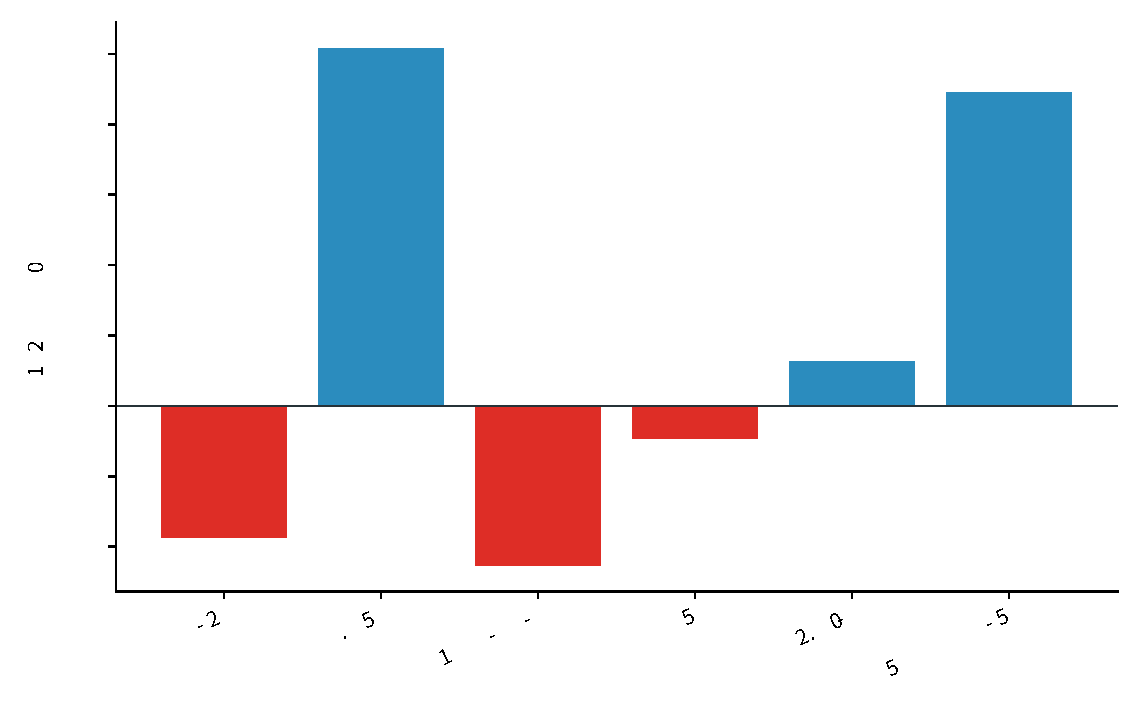
\includegraphics[width=\linewidth]{figures/per_class_evidence_gain.pdf}
  \caption{不同证据配置的逐类别候选判断增益}
  \label{fig:per_class_evidence_gain}
\end{figure}

\subsection{RQ2：端到端纠错}
\label{subsec:rq2}

RQ2比较八种端到端设置。B0以0.001低阈值保留完整检测排序，只用于mAP参考。B1是验证集选择的检测器工作点。B2只使用ECC、SSIM、形态学差异候选和冻结拓扑规则，不调用验证器。B7对抽样候选全量复核且不使用门控，B8采用手工线性风险门。Full采用学习式Logistic复检门、分动作接受门和安全规则。Oracle-C在完整固定候选集上按真值选择最优动作，反映候选覆盖上界。Oracle-A只在已有真实验证器输出的候选中接受正效用动作，反映当前提议动作集合的接受上界。

五折固定候选共51222个，超过既定调用上限。实验在每折按原始错误类型和候选来源比例分层抽样800个候选，共评价约4000个候选。未抽中的候选保持B1输出。抽样比例从fold\_0的5.5348\%到fold\_4的12.5156\%。所有方法共享同一批A2响应，B7、B8和Full之间的差异来自门控而非调用样本变化。表~\ref{tab:rq2_main}报告五折均值与折间标准差。

\begin{table*}[t]
  \centering
  \caption{RQ2五折端到端结果}
  \label{tab:rq2_main}
  \setlength{\tabcolsep}{5pt}
  \begin{tabular}{lcccc}
    \hline
    方法 & F1 & mAP@0.5 & TPRR & HCR \\
    \hline
    B0$^{\dagger}$ & $0.2871\pm0.0813$ & $0.9491\pm0.0205$ & 不适用 & 不适用 \\
    B1 & $0.9118\pm0.0344$ & $0.8813\pm0.0575$ & 不适用 & 不适用 \\
    B2 & $0.0014\pm0.0011$ & $0.0001\pm0.0002$ & 不适用 & 不适用 \\
    B7 & $0.8660\pm0.0368$ & $0.8246\pm0.0655$ & $0.9572\pm0.0174$ & $0.9326\pm0.0280$ \\
    B8 & $0.8787\pm0.0471$ & $0.8450\pm0.0867$ & $0.9717\pm0.0305$ & $0.9607\pm0.0456$ \\
    Full & $0.9117\pm0.0343$ & $0.8810\pm0.0573$ & $0.9998\pm0.0003$ & $0.4000\pm0.5477$ \\
    Oracle-C & $0.9555\pm0.0254$ & $0.9106\pm0.0471$ & 不适用 & 不适用 \\
    Oracle-A & $0.9143\pm0.0336$ & $0.8826\pm0.0573$ & $1.0000\pm0.0000$ & $0.0000\pm0.0000$ \\
    \hline
  \end{tabular}
  \vspace{2pt}
  \parbox{0.95\textwidth}{\footnotesize $^{\dagger}$B0使用0.001低阈值保留检测排序，其F1只描述该阈值下的输出，不作为部署工作点结论。}
\end{table*}

B2的F1只有0.0014，说明确定性差异规则不能单独替代检测器。无门控B7把F1从B1的0.9118降至0.8660，HCR达到0.9326。绝大多数已执行修改降低了检测效用。手工线性门B8的F1为0.8787，仍低于B1，HCR为0.9607。缺少动作级安全约束时，验证器输出不能作为可靠的后置纠错结果。

Full的F1为$0.9117\pm0.0343$，B1为$0.9118\pm0.0344$。按图像聚类的配对bootstrap给出总体F1差值$-0.000064$。95\%置信区间为$[-0.000273,+0.000094]$，区间跨越0。Full与B1无统计差异，完整流程未获得可辨别的端到端净提升。小数点后的波动不能表述为性能改进。Full的TPRR达到0.9998，学习式双门控基本保留了原始正确检测。HCR均值为0.4000，折间标准差为0.5477。实际接受动作很少，个别折的一次有害动作会使该折比率大幅变化。因此，安全性需要结合绝对动作计数解释。

图~\ref{fig:error_transfer}和表~\ref{tab:error_transfer}给出错误转移。约4000个评价候选中，48个原始误报只纠正1个，47个未纠正。36个漏检均未恢复，6个错分类均未修正。734个原始正确检测中，732个保持正确，2个被误删。3174个差异噪声候选和2个纯定位错误也均未纠正。Full未发生误改类别、差异候选新增误报或将错误类别改成另一错误类别，实际损失均来自2次误删TP。双门控大幅减少了有害修改，但几乎没有放行有效修正。

\begin{table}[t]
  \centering
  \caption{Full候选级错误转移计数}
  \label{tab:error_transfer}
  \setlength{\tabcolsep}{4pt}
  \begin{tabular}{lrrrr}
    \hline
    原始类型 & 保持正确 & 已纠正 & 未纠正 & 误删 \\
    \hline
    误报 & 0 & 1 & 47 & 0 \\
    漏检 & 0 & 0 & 36 & 0 \\
    错分类 & 0 & 0 & 6 & 0 \\
    正确检测 & 732 & 0 & 0 & 2 \\
    \hline
  \end{tabular}
\end{table}

\begin{figure}[t]
  \centering
  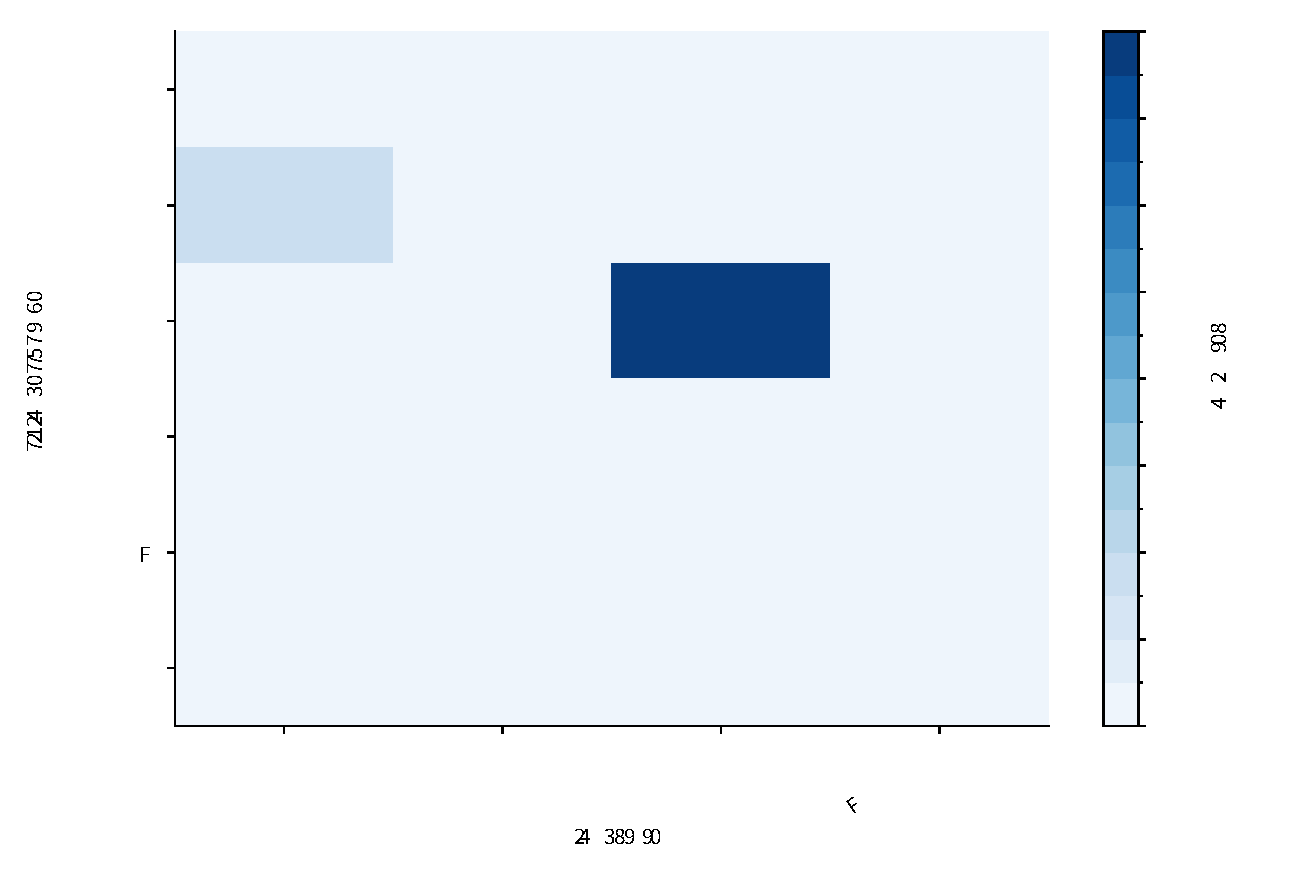
\includegraphics[width=\linewidth]{figures/error_transfer_heatmap.pdf}
  \caption{Full方法的候选级错误转移热图}
  \label{fig:error_transfer}
\end{figure}

Oracle结果用于定位限制因素。Oracle-C的F1为0.9555，相对B1保留约0.044的提升空间，说明固定候选集仍有纠错潜力。Oracle-A只接受真实验证器输出中的正效用动作，F1也仅为0.9143，相对B1提高0.0025。即使接受决策达到理想状态，当前提议动作仍远未达到候选上界。B1与Oracle-C之间的大部分空间损失在验证器判断阶段，而非复检门或接受门。RQ2表明双门控大幅减少了有害修改，但端到端净收益接近零。当前主要限制因素是多模态验证器对工业细粒度缺陷的判断质量。

\subsection{RQ3：门控效率与可靠性}
\label{subsec:rq3}

RQ3在RQ2的同一批A2缓存上离线回放六种策略和六个预算点。预算是每折800个抽样候选中的调用比例，取5\%、10\%、20\%、40\%、60\%和100\%。random按固定随机种子抽样，low\_confidence按检测置信度排序。manual\_linear使用手工线性风险分数。logistic和lightgbm使用学习式复检分数排序。review\_acceptance在logistic排序后执行接受门与安全规则。表~\ref{tab:rq3_budget}列出全部36个组合的五折均值，RR表示错误候选复核召回率。

\begin{table*}[t]
  \centering
  \caption{六种门控策略在六个调用预算下的结果，数值为五折均值}
  \label{tab:rq3_budget}
  \setlength{\tabcolsep}{3.5pt}
  \begin{tabular}{llrrrrrr}
    \hline
    策略 & 指标 & 5\% & 10\% & 20\% & 40\% & 60\% & 100\% \\
    \hline
    random & F1 & 0.9088 & 0.9067 & 0.9015 & 0.8915 & 0.8820 & 0.8660 \\
           & HCR & 0.9633 & 0.9471 & 0.9342 & 0.9382 & 0.9335 & 0.9326 \\
           & RR & 0.0315 & 0.1322 & 0.2251 & 0.3951 & 0.5763 & 1.0000 \\
    \hline
    low\_confidence & F1 & 0.9116 & 0.9112 & 0.9096 & 0.9055 & 0.9013 & 0.8660 \\
           & HCR & 0.6000 & 0.8000 & 1.0000 & 1.0000 & 0.9935 & 0.9326 \\
           & RR & 0.0000 & 0.0000 & 0.0065 & 0.0769 & 0.2048 & 1.0000 \\
    \hline
    manual\_linear & F1 & 0.9106 & 0.9096 & 0.9077 & 0.9032 & 0.8989 & 0.8660 \\
           & HCR & 1.0000 & 1.0000 & 0.9913 & 0.9913 & 0.9812 & 0.9326 \\
           & RR & 0.0129 & 0.0614 & 0.1644 & 0.2820 & 0.4614 & 1.0000 \\
    \hline
    logistic & F1 & 0.9076 & 0.9006 & 0.8942 & 0.8856 & 0.8782 & 0.8660 \\
           & HCR & 0.6813 & 0.8059 & 0.8697 & 0.8977 & 0.9156 & 0.9326 \\
           & RR & 0.4649 & 0.5103 & 0.6686 & 0.8397 & 0.9347 & 1.0000 \\
    \hline
    lightgbm & F1 & 0.9094 & 0.9050 & 0.8966 & 0.8838 & 0.8744 & 0.8660 \\
           & HCR & 0.6597 & 0.7708 & 0.8452 & 0.8960 & 0.9158 & 0.9326 \\
           & RR & 0.6236 & 0.7455 & 0.8562 & 0.9230 & 0.9700 & 1.0000 \\
    \hline
    review\_acceptance & F1 & 0.9117 & 0.9116 & 0.9115 & 0.9115 & 0.9115 & 0.9115 \\
           & HCR & 0.4000 & 0.4000 & 0.4000 & 0.4000 & 0.4000 & 0.4000 \\
           & RR & 0.4649 & 0.5103 & 0.6686 & 0.8397 & 0.9347 & 1.0000 \\
    \hline
  \end{tabular}
\end{table*}

复检门的排序效率在低预算区间最清楚。5\%预算下，Logistic复检门覆盖46.49\%的错误候选，随机策略仅覆盖3.15\%，前者约为后者的14.8倍。LightGBM在同一预算达到62.36\%。其PR AP为0.4311，高于Logistic的0.1839。端到端实验按预注册协议固定使用Logistic主模型，未依据测试结果更换。低置信度策略在5\%和10\%预算下的错误候选复核召回均为0。检测置信度不能替代针对“是否值得复核”训练的风险分数。复检门将有限调用集中到潜在可纠错位置，但不保证验证器修改正确。

接受门决定预算扩大后是否退化。不使用接受门时，随机回放的F1从5\%预算的0.9088降至100\%预算的0.8660，累计下降0.0428。20\%和60\%预算下分别为0.9015和0.8820。加入接受门后，F1从5\%预算的0.9117变为20\%、60\%和100\%预算下约0.9115。各预算结果与B1无统计差异，保持在基线水平。该稳定性来自多数提议未被执行，不代表验证器判断改善。HCR维持0.4000仍需结合RQ2中的极少接受动作解释，不能作为充分校准的概率保证。

调用成本随预算近似线性增加。六种策略在相同预算下调用数一致。每图调用次数从5\%预算的$0.1341\pm0.0118$增至100\%预算的$2.6821\pm0.2363$。真实缓存记录给出的单候选平均时延约29.1秒，跨策略与预算的P95最高约41.4秒。每图输入token数在logistic的5\%预算下为$123.35\pm10.64$。该数值在100\%预算下增至$2518.81\pm223.24$。在当前后端吞吐下，全量复核会降低F1并增加调用成本。低预算复检门控制调用量，接受门控制动作风险。

图~\ref{fig:rq3_curves}给出F1、HCR与调用率曲线。图~\ref{fig:acceptance_reliability}给出接受门可靠性分析。可靠性图的横轴为预测概率，纵轴为观测正效用率。曲线多处偏离理想对角线，与抽样动作上的校准不稳定一致。门控曲线显示复检门提高错误覆盖效率，接受门控制已执行动作的风险。只有复检门时，高风险候选更快进入复核，但错误提议仍使F1下降。只有接受门时，系统能减少有害修改，却不能降低验证器调用成本。因此，两道门承担不同任务。

\begin{figure*}[t]
  \centering
  \begin{minipage}{0.48\textwidth}
    \centering
    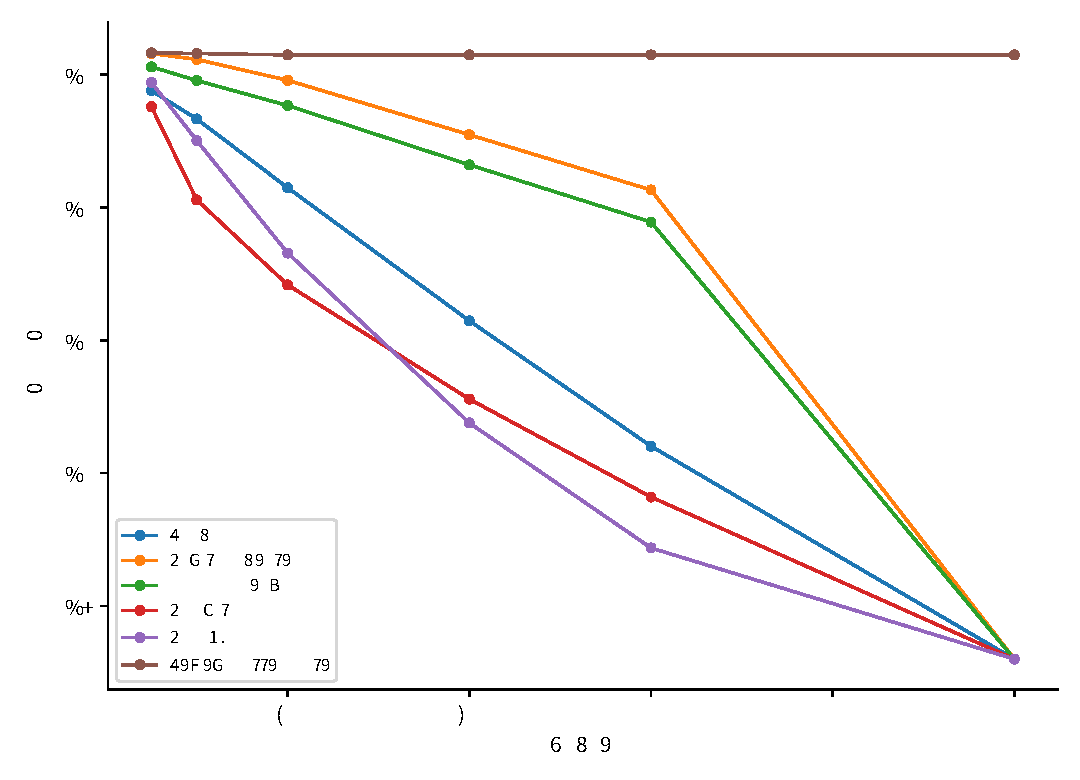
\includegraphics[width=\linewidth]{figures/f1_call_rate.pdf}
    \small (a) F1与调用率
  \end{minipage}\hfill
  \begin{minipage}{0.48\textwidth}
    \centering
    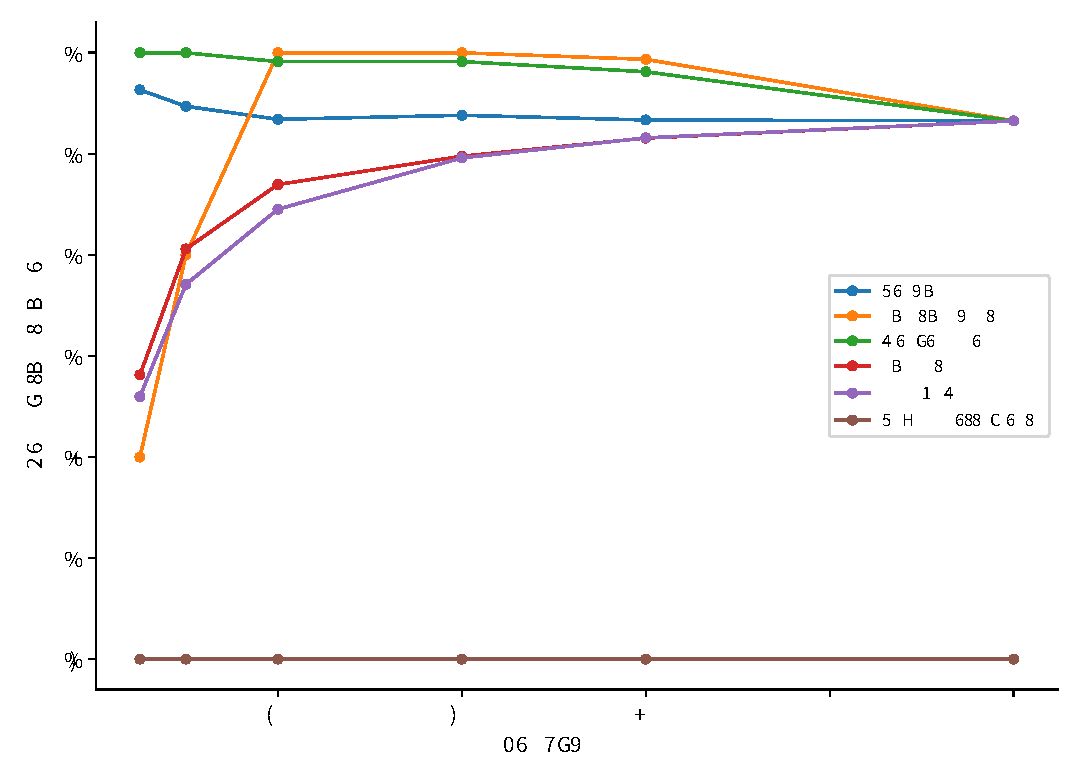
\includegraphics[width=\linewidth]{figures/hcr_call_rate.pdf}
    \small (b) HCR与调用率
  \end{minipage}
  \caption{不同门控策略的性能、风险与调用预算关系}
  \label{fig:rq3_curves}
\end{figure*}

\begin{figure}[t]
  \centering
  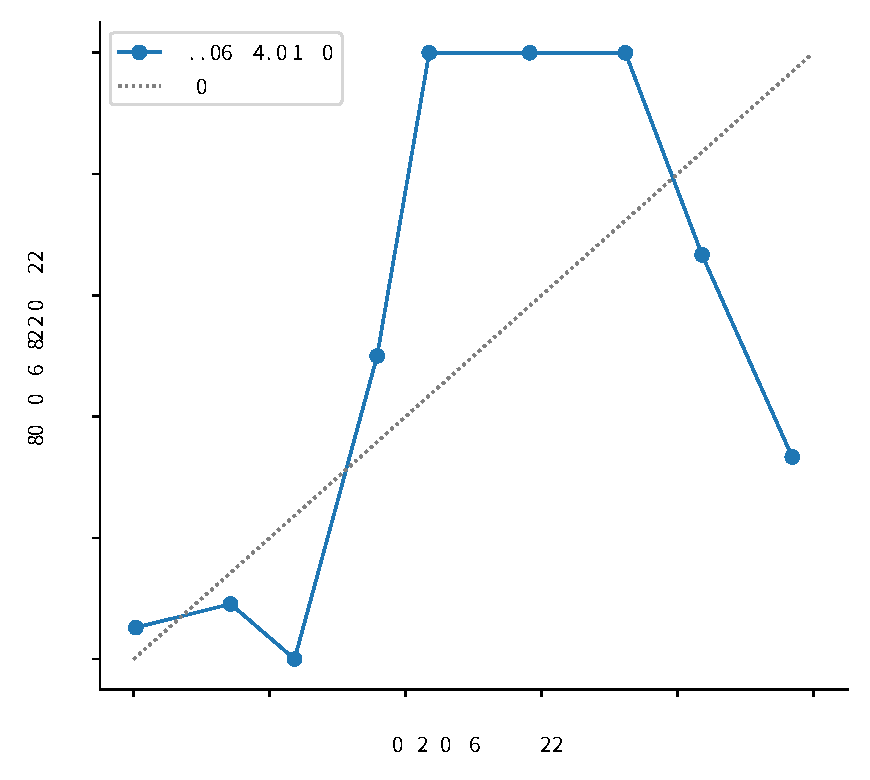
\includegraphics[width=\linewidth]{figures/acceptance_reliability.pdf}
  \caption{接受门的可靠性分析}
  \label{fig:acceptance_reliability}
\end{figure}

\subsection{RQ4：鲁棒性与模型替换}
\label{subsec:rq4}

RQ4在fold\_0的325张测试图像上进行。几何扰动施加于正常模板，光度扰动施加于待检图。每个条件重新计算配准、光度归一、外观残差、骨架差异和差异候选。几何实验组合无二次配准或ECC配准、直接XOR或容差XOR，以及是否使用配准质量阈值。这些组合共产生8775条图像与扰动条件评价记录。fold\_0共有343个基础漏检。漏检恢复率以完整测试折为分母，定义为差异候选与未覆盖真值框达到IoU不低于0.3的比例。最终F1和HCR使用fold\_0的800个真实A2结论冻结回放，只重算扰动影响的证据与门控特征。该协议隔离了配准证据退化，但不等价于在每种扰动下重新调用验证器。

\subsubsection{容差XOR与配准质量}

无额外扰动时，ECC加直接XOR恢复23个漏检，恢复率为$23/343=6.71\%$。改用容差XOR后恢复81个，达到$81/343=23.62\%$，提升约3.5倍。XOR伪差异像素占比同时从0.02892降至0.01441，降低约50\%。容差操作允许骨架在小邻域内匹配，从而压制JPEG边缘和亚像素错位产生的双边轮廓。表~\ref{tab:rq4_xor}表明，恢复率提高并未增加伪差异面积。

\begin{table}[t]
  \centering
  \caption{无额外扰动时直接XOR与容差XOR比较}
  \label{tab:rq4_xor}
  \setlength{\tabcolsep}{4pt}
  \begin{tabular}{lrr}
    \hline
    设置 & 漏检恢复率 & XOR占比 \\
    \hline
    ECC+直接XOR & 23/343=6.71\% & 0.02892 \\
    ECC+容差XOR & 81/343=23.62\% & 0.01441 \\
    \hline
  \end{tabular}
\end{table}

在同方向正平移序列中，$q_{\mathrm{reg}}$均值随扰动增大而下降。无扰动、平移2像素和平移8像素时，均值分别为0.8599、0.8410和0.7992。对应$q_{\mathrm{reg}}<0.5$的比例为4.00\%、4.62\%和4.92\%。该受控序列说明质量分能响应逐渐增强的错位。平移8像素时，完整设置的F1为0.8796，HCR为1.0000。相关强扰动条件只有1个被接受动作，且该动作有害。HCR为1不表示大量候选受到破坏，只说明这一次放行动作失败。

配准质量阈值的保护作用未获实证。全部几何条件中，冻结阈值0.5没有拦截任何有害动作，因为相关候选的$q_{\mathrm{reg}}$均未低于阈值。$q_{\mathrm{reg}}$同时惩罚估计变换幅度。ECC修正真实初始错位后，其分数有时低于以恒等变换计算的代理分数。本实验只支持$q_{\mathrm{reg}}$在选定平移强度序列中的下降趋势，不支持它在所有几何扰动间严格单调。当前阈值也未形成可靠的风险保证。该负面结果与容差XOR的收益属于不同结论。

光度扰动包括亮度$\pm10$、$\pm20$，对比度0.8和1.2，两档噪声以及两档模糊。完整设置在这些条件下的最终F1均为0.8803，HCR均为0。DeepPCB像素主要集中在0和255附近，较小光度变化的区分度有限。该结果只说明冻结回放协议下没有触发额外有害修改，不能推广为对任意成像变化鲁棒。图~\ref{fig:rq4_registration}汇总了XOR表示、配准质量分布和配准扰动性能。

\begin{figure*}[t]
  \centering
  \begin{minipage}{0.32\textwidth}
    \centering
    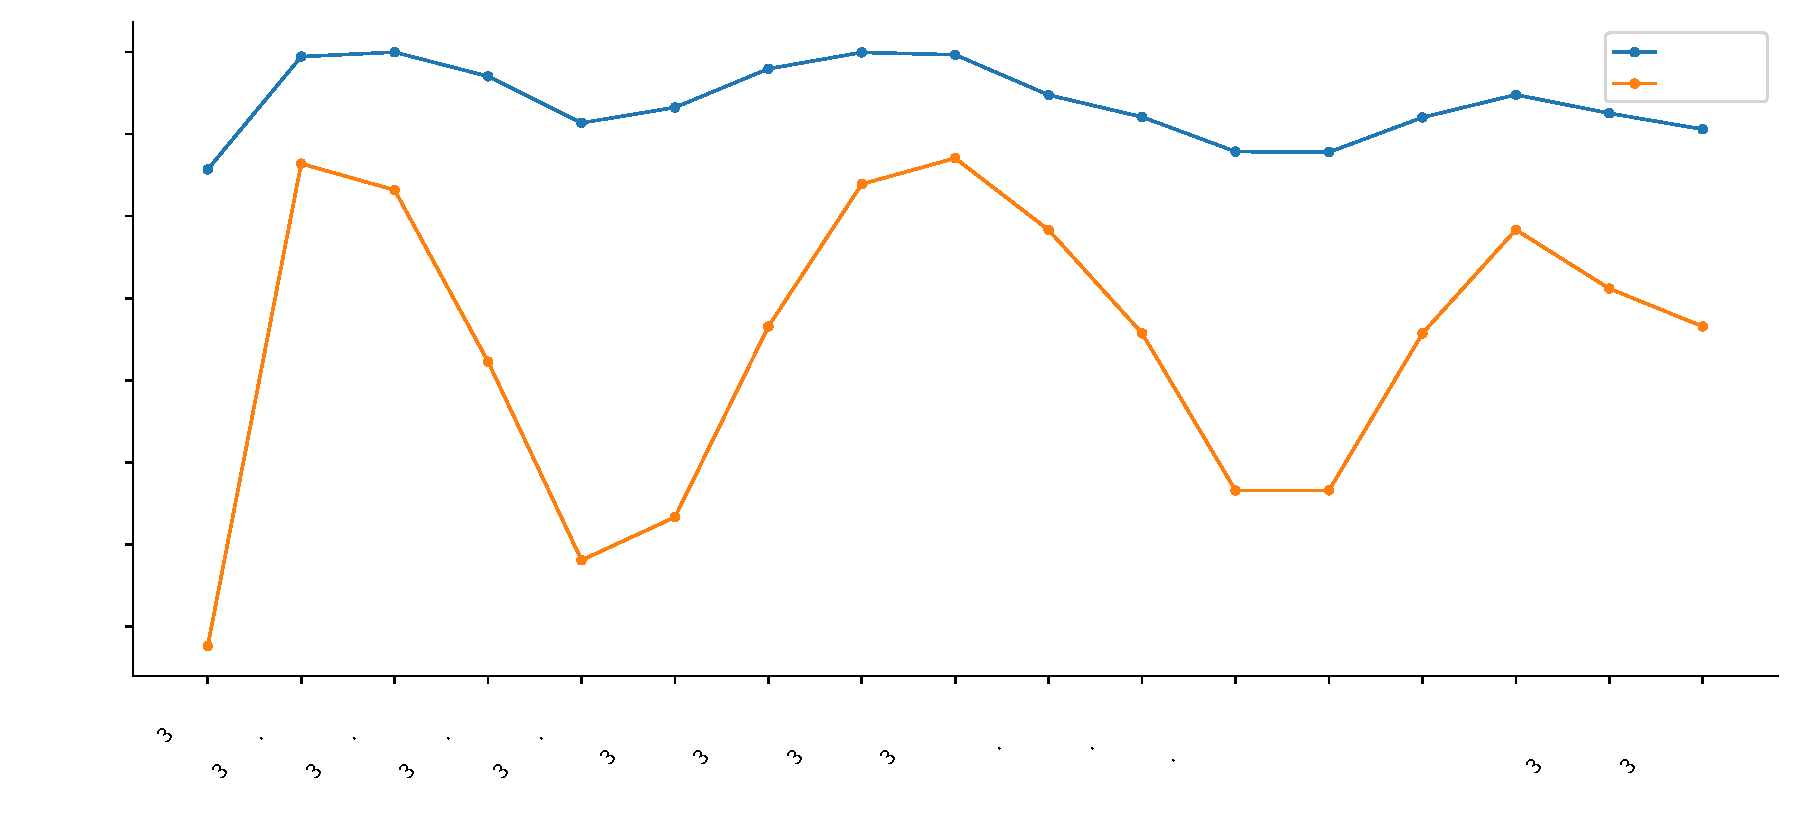
\includegraphics[width=\linewidth]{figures/rq4_xor_comparison.pdf}
    \small (a) XOR表示比较
  \end{minipage}\hfill
  \begin{minipage}{0.32\textwidth}
    \centering
    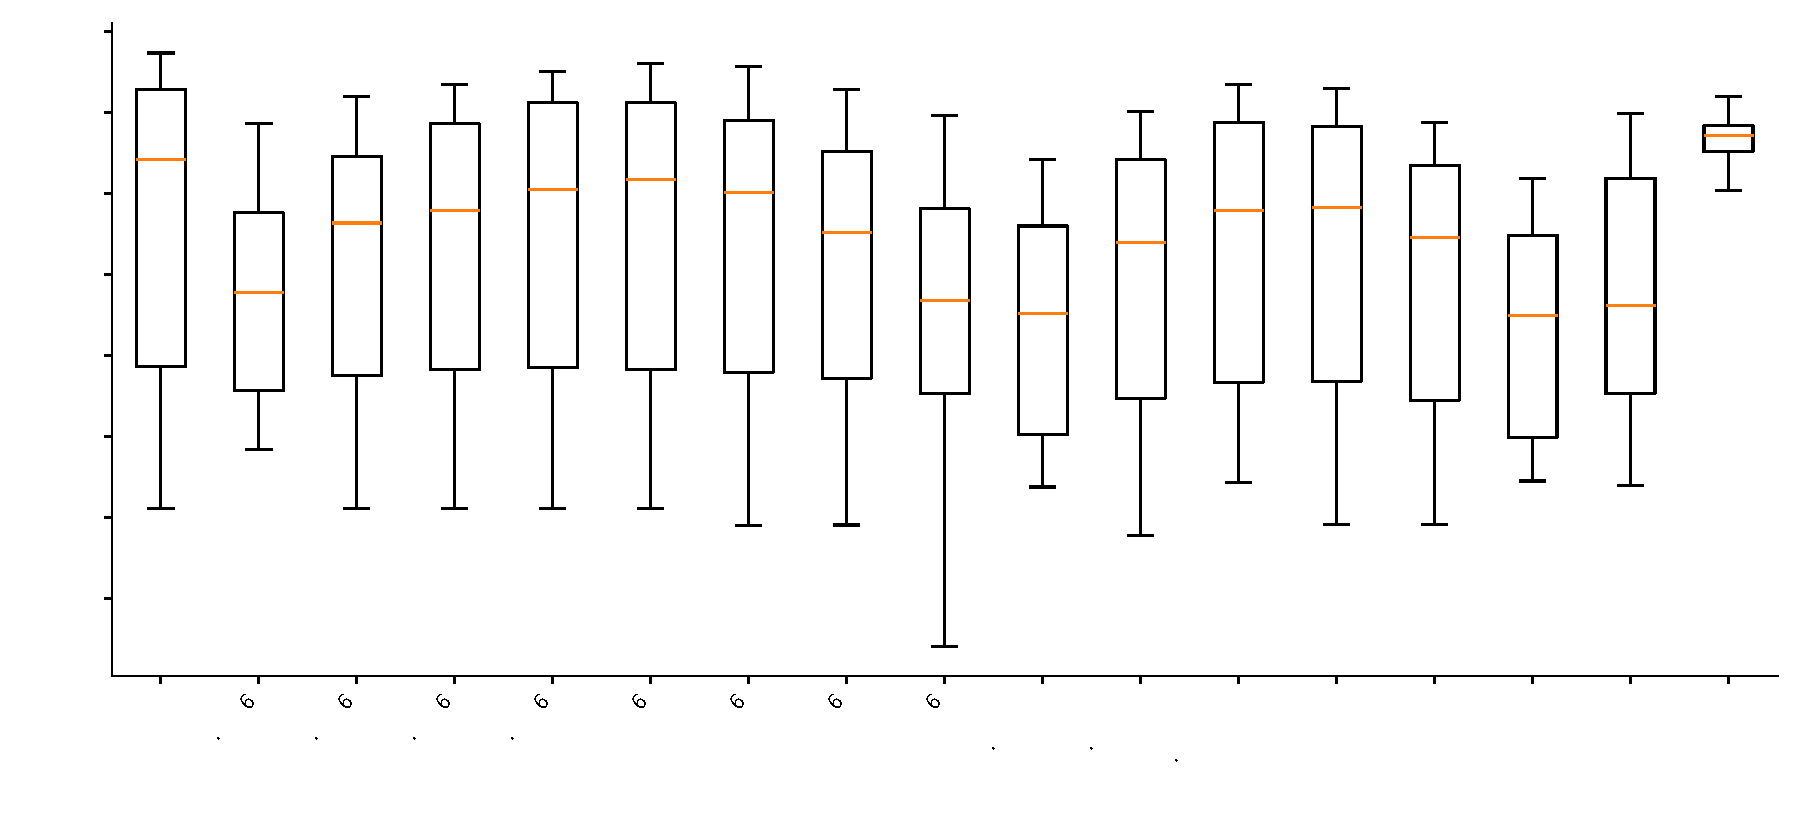
\includegraphics[width=\linewidth]{figures/rq4_qreg_distribution.pdf}
    \small (b) 配准质量分布
  \end{minipage}\hfill
  \begin{minipage}{0.32\textwidth}
    \centering
    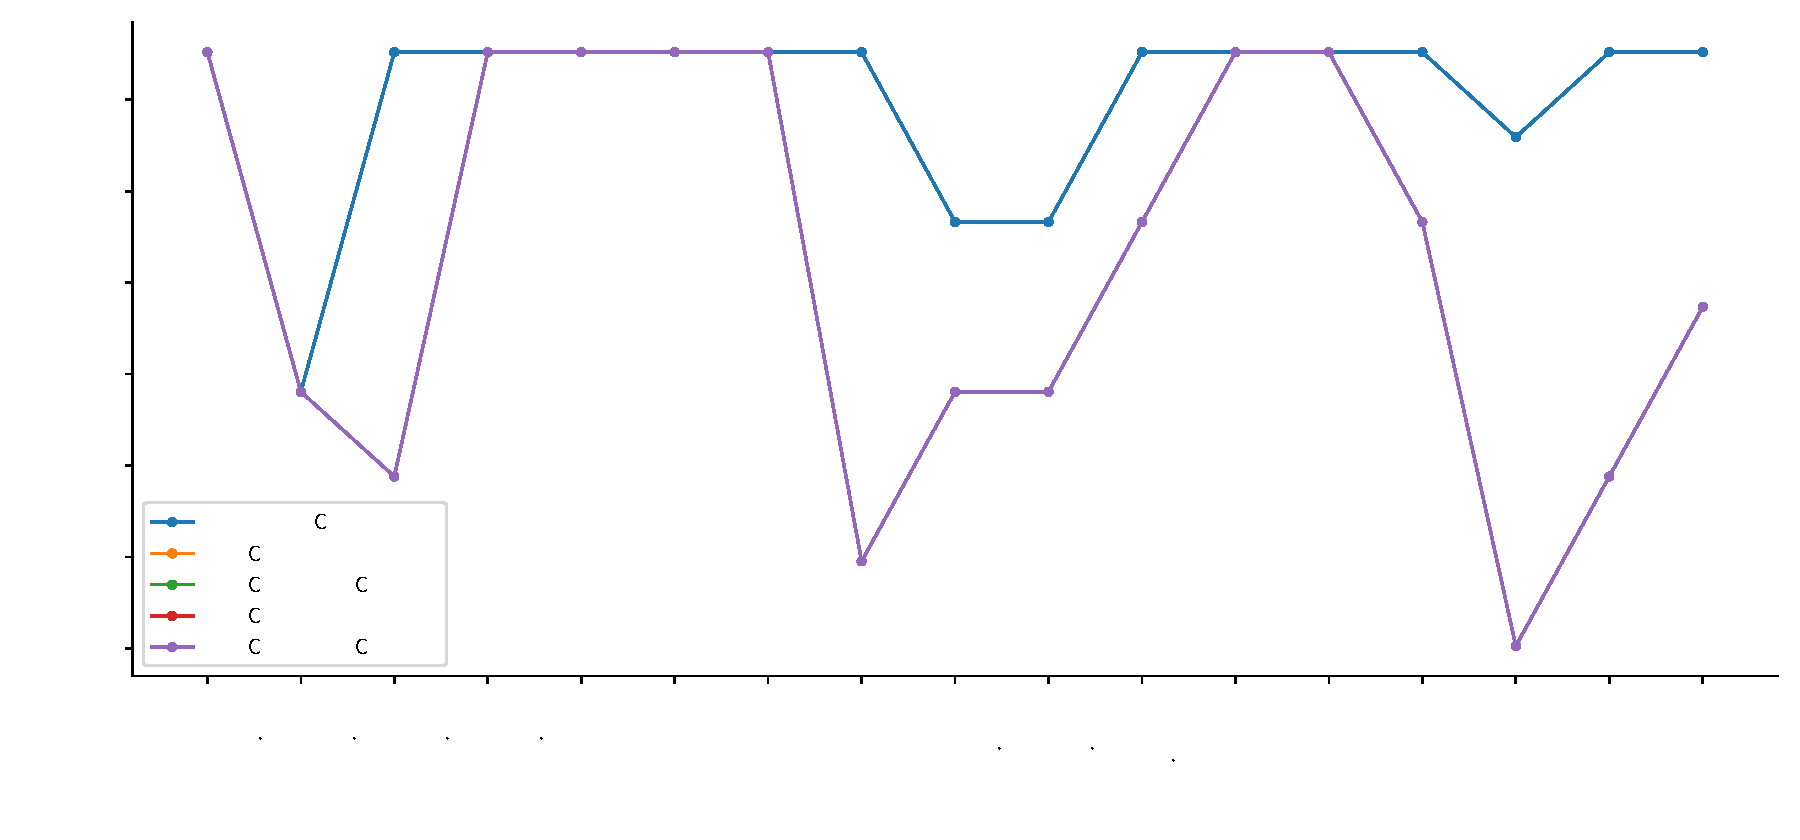
\includegraphics[width=\linewidth]{figures/rq4_registration_performance.pdf}
    \small (c) 配准扰动性能
  \end{minipage}
  \caption{配准扰动、质量分与容差XOR的鲁棒性结果}
  \label{fig:rq4_registration}
\end{figure*}

\subsubsection{检测器与门控模型替换}

检测器替换采用官方PekingU RT-DETR-R18VD。模型在fold\_0训练后预测全部测试图像，并对200个比例分层候选调用A2验证器。表~\ref{tab:rq4_model}显示，RT-DETR-R18VD基线F1为0.6416，mAP@0.5为0.6483。二者均低于YOLOv8s五折工作点。完整流程实际调用12次，但没有接受任何修改。最终F1仍为0.6416，HCR为0。该对照没有出现性能退化。由于系统未执行动作，结果不能证明双门控在检测器替换时有效，也不能证明流程能改善不同架构的检测性能。

门控模型替换也限制在fold\_0的200个分层候选上。Logistic在验证阈值0.208300下调用0次。LightGBM在阈值0.145905下调用3次。两者最终F1均为0.8803，HCR均为0。调用数过少，无法比较两种模型的纠错能力，也不足以验证安全规则对门控分类器变化的稳健性。

\begin{table}[t]
  \centering
  \caption{RQ4检测器替换结果}
  \label{tab:rq4_model}
  \setlength{\tabcolsep}{4pt}
  \begin{tabular}{lrrr}
    \hline
    设置 & F1 & mAP@0.5 & HCR \\
    \hline
    RT-DETR-R18VD基线 & 0.6416 & 0.6483 & 不适用 \\
    RT-DETR-R18VD+完整流程 & 0.6416 & 0.6483 & 0.0000 \\
    \hline
  \end{tabular}
\end{table}

第二个多模态验证器后端未完成对照，HRIPCB也未纳入实验。RQ4支持的确定性发现是：容差XOR在DeepPCB fold\_0上提高漏检候选恢复率，并减少伪差异。RT-DETR-R18VD对照中没有接受任何修改，因而只能报告未发生有害动作。跨检测器增益、跨数据集泛化和跨验证器一致性均超出当前证据范围。

\subsection{讨论与局限}
\label{subsec:discussion_limitations}

四个研究问题给出一致的能力边界。正常模板提高了验证器的候选存在性判断，完整外观与拓扑证据没有稳定增量。双来源候选保留了Oracle-C上界，真实验证器输出对应的Oracle-A增益只有0.0025。复检门能在低预算下集中覆盖错误候选，接受门使各预算结果与基线无统计差异。端到端Full仍未超过基础工作点。当前实验支持风险受控的复核流程，不支持稳定提高检测指标的结论。以下四项局限限定了结论范围。

第一项局限是接受门的训练分布与部署提议分布不完全匹配。训练阶段的remove、relabel和add提议由冻结的确定性证据代理生成，正效用标签由折外检测和真值计算。端到端部署的提议则来自真实验证器。两类提议的类别频率、错误模式和分数分布存在差异风险，可能造成接受概率失配。该问题直接影响HCR、动作召回和阈值可靠性，也能解释接受门过度保守以及Oracle-A高于Full的部分差距。它不影响YOLOv8s基础检测指标、RQ1的证据输入比较和Oracle-C候选覆盖结论。后续实验需使用已积累的约7000次真实调用重训接受门，并在独立模板组上重新校准阈值。

第二项局限是实验只有一个真实多模态验证器后端。RQ1的证据偏好、自由文本解析失败、标签可见对照和RQ2的Oracle-A上限均基于\texttt{gpt-5.6-sol}。当前结果只支持“该后端在本协议下判断质量不足”，不能推广到所有视觉语言模型。检测器替换不能弥补这一缺口，因为验证器保持不变。该局限影响所有涉及验证器正确率和提示行为的结论。数据泄漏判断、基础错误分解、容差XOR的确定性候选结果和调用成本实测不受此限制。

第三项局限来自RQ2的分层抽样评价。五折固定候选总数为51222，每折只调用800个，覆盖比例为5.5\%至12.5\%。未抽中的候选保持B1输出。该协议能在调用预算内公平比较B7、B8和Full，也能精确计数抽样区域内的错误转移。大量未修改候选会稀释端到端净收益，稀有正确动作也可能未进入样本。Full相对B1的bootstrap区间只描述本抽样与冻结响应协议，不等于全量调用51222个候选后的区间。Oracle-C使用完整固定候选集，仍可判断候选覆盖潜力。Oracle-A、FPCR、MDRR、MCCA和错误转移矩阵均受抽样范围约束。

第四项局限是fold\_0测试集只包含group20085一个模板组。该折有325对图像，样本量最大，但板型多样性最低。RQ4主要在该折执行，其扰动结果会受到单一模板结构特征的影响。五折总体检测与RQ2主表仍覆盖全部11个模板组。fold\_0的单组性质主要限制RQ4配准趋势、RT-DETR替换和门控替换的外推范围。后续实验需在其余四折重复关键扰动，并按模板组汇总$q_{\mathrm{reg}}$和漏检恢复率。这些实验将检验容差XOR收益是否为group20085特有现象。

官方划分存在模板泄漏，按模板组隔离是主结论成立的前提。正常模板和学习式复检排序分别获得证据消融与低预算覆盖率的支持。接受门使各预算结果保持在基线水平，但Full的HCR仍为0.4000，并有2次误删TP。完整证据卡与去锚定协议没有显示稳定优势。Oracle-C与Oracle-A的差距表明，当前主要限制因素是验证器判断质量。Full与B1无统计差异，端到端净收益接近零。
